\documentclass[tikz,border=10pt]{standalone}
\usepackage[utf8]{inputenc}
\usepackage[T1]{fontenc}
\usepackage[english]{babel}
\usepackage{graphicx}
\usepackage{amsmath,amssymb}
\usepackage{tikz}
\usepackage{hyperref}
\usepackage{geometry}
\usepackage{fancyhdr}
\usepackage{listings}
\usepackage{color}
\usepackage{caption}
\usepackage{booktabs}
\usepackage{longtable}
\usepackage{float}
\usepackage{array}
\usepackage{subfigure}
\usepackage{multirow}
\usepackage{multicol}
\usepackage[acronym]{glossaries}
\usepackage{xcolor}
\usetikzlibrary{shapes.geometric,arrows,positioning,calc,fit}

\begin{document}
\pagecolor{white}
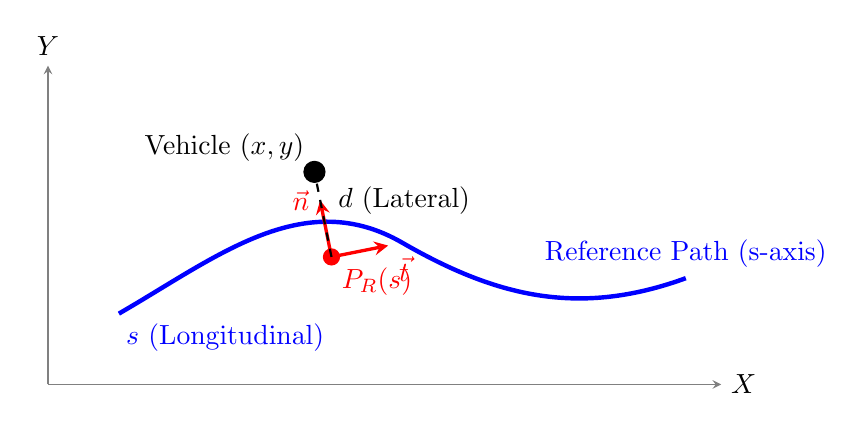
\begin{tikzpicture}[>=stealth, scale=0.9, thick]
    % Cartesian axes
    \draw[->, gray, thin] (-1,-1) -- (8.5,-1) node[right, black] {$X$};
    \draw[->, gray, thin] (-1,-1) -- (-1,3.5) node[above, black] {$Y$};
    
    % Reference centerline curve
    \draw[blue, ultra thick] (0,0) to[out=30, in=150] (4,1) to[out=-30, in=200] (8,0.5);
    \node[blue, above] at (8,0.5) {Reference Path (s-axis)};
    
    % Vehicle position
    \filldraw[black] (2.76, 2.0) circle (4pt) node[above left] {Vehicle $(x, y)$};
    
    % Projection point on reference path
    \filldraw[red] (3.0, 0.8) circle (3pt) node[below right] {$P_R(s)$};
    
    % Tangent and Normal vectors at PR
    \draw[->, red, very thick] (3.0, 0.8) -- (3.8, 0.96) node[below right] {$\vec{t}$};
    \draw[->, red, very thick] (3.0, 0.8) -- (2.84, 1.6) node[left] {$\vec{n}$};
    
    % Projection line representing d
    \draw[dashed, black] (3.0, 0.8) -- (2.76, 2.0);
    \node[right] at (2.95, 1.6) {$d$ (Lateral)};
    
    % Longitudinal coordinate s
    \node[blue, below] at (1.5, 0.0) {$s$ (Longitudinal)};
\end{tikzpicture}
\end{document}